\chapter{Case Study 2: A Telecoms Language}

\section{Introduction}

This chapter presents an example of the definition of a domain
specific modelling language: a telecoms modelling language. The
approach taken is to extend the XCore metamodel and to use package
extension and metapackages to construct stereotyped concrete
syntax elements for the language. Mappings are then constructed
from the language metamodel to a metamodel of Java and a metamodel
of a user interface language. The work presented in this chapter
is based on an earlier case study described in
\cite{ossjcasestudy}.

\section{The Case Study: OSS/J Inventory}

Developing and operating Operational Support Systems (OSS) for
telecommunications companies (telcos) is a very expensive process
whose cost continuously grows year on year. With the introduction
of new products and services, telcos are constantly challenged to
reduce the overall costs and improve business agility in terms of
faster time-to-market for new services and products. It is
recognised that the major proportion of overall costs is in
integration and maintenance of OSS solutions. Currently, the OSS
infrastructure of a typical telco comprises an order of O(1000)
systems all with point-to-point interconnections and using diverse
platforms and implementation technologies. The telcoms OSS
industry has already established the basic principles for building
and operating OSS through the TMF NGOSS programme [NGOSS] and the
OSS through Java initiative \cite{ossj}. In summary, the NGOSS
applies a top-level approach through the specification of an OSS
architecture where:

\begin{itemize}
\item Technology Neutral and Technology Specific Architectures are
separated. \item The more dynamic "business process" logic is
separated from the more stable "component" logic. \item Components
present their services through well defined "contracts" \item
"Policies" are used to provide a flexible control of behaviour in
an overall NGOSS system. \item The infrastructure services such as
naming, invocation, directories, transactions, security,
persistence, etc are provided as a common deployment and runtime
framework for common use by all OSS components and business
processes over a service bus.
\end{itemize}

The case-study was based upon OSS component APIs specified in Java
and J2EE by OSS/J. The case-study was specifically driven by the
OSS/J Inventory component API \cite{Gauthier} and set as its goal
to automatically conduct compliance tests between the API
specification and the results of the case study. This end acquired
more value by the fact that this particular API specification
lacks, as of yet, a reference implementation and compatibility kit
that would permit its practical validation.

The exercise had two main objectives:

\begin{itemize}
\item Construction of a domain specific language metamodel for the
OSS/J Inventory: The OSS/J Inventory specification document
includes a UML class diagram of an inventory meta-model and some
textual, i.e. informal, description of its semantics. The
meta-model defines the types of information/content the inventory
will manage, such as products, services and resources. \item
Automatic generation of a system implementation conforming to
standard OSS/J architectural patterns and design guidelines: In
order to comply with the OSS/J guideline, the case-study aims at
implementing an application tool that allows users to manage the
inventory content through a simple GUI. Example users of such a
tool may be front-desk operators who respond to customer calls and
access the inventory to setup a new or change the state of an
existing product/service instance.
\end{itemize}

Figure \ref{inventoryoverview} shows how a language definition for
the inventory modelling language was constructed. Firstly, a
metamodel for the inventory DSL was defined by extending the XCore
meta-model. XOCL was used to specify meta-model constraints so
that models written in the inventory language can be checked for
correctness. That is, by means of XOCL, the meta-model semantics
can be formally captured and automatically enforced, in contrast
to the informal, textual description of the semantics presented in
the OSS/J Inventory API specification document. Next, mapping
rules written in XMap were constructed to transform the inventory
meta-model into meta-models of two target platform specific
languages: EJB and Java.

\begin{figure}[htb]
\begin{center}
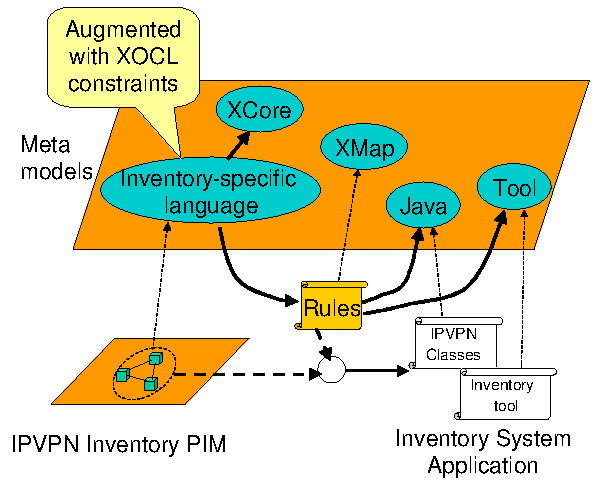
\includegraphics[width=12cm]{CaseStudy2/figures/inventoryoverview.pdf}
\caption{Overview of the inventory language definition}
\label{inventoryoverview}
\end{center}
\end{figure}

\section{Abstract Syntax Model}

Figure \ref{inventoryas} shows the abstract syntax model for the
inventory language. As mentioned earlier, it includes concepts
from the OSS/J Core Business Entities, which are a subset of TMF's
NGOSS standard. The inventory language consists of the following
constructs:

\begin{itemize}
\item Entity, that represents any type of information included in
the inventory. According to the specification, three types of
inventory content are defined, namely, Product, Service and
Resource, which extend type Entity. \item   EntitySpecification,
that represents configurations of Entities, i.e. constraints, such
as range of values or preconfigured setting on features of the
Entity. Again, the API specification defines three subtypes of
EntitySpecification, namely, ProductSpecification,
ServiceSpecification and ResourceSpecification, each representing
specifications for Service, Product and Resource, respectively. �
EntityAttribute, that represents relationships between Entity
types.
\end{itemize}

\begin{figure}[htb]
\begin{center}
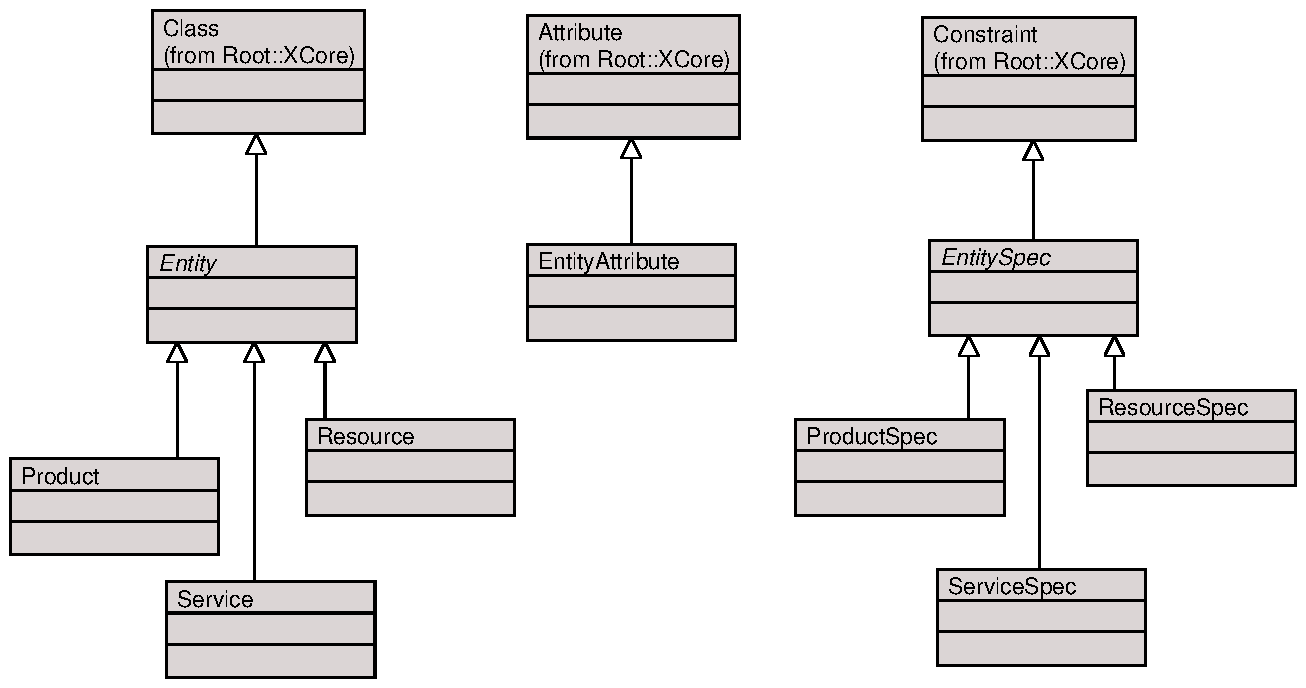
\includegraphics[width=14cm]{CaseStudy2/figures/abstractsyntax.pdf}
\caption{The abstract syntax model for the inventory language}
\label{inventoryas}
\end{center}
\end{figure}

A number of concepts from the XCore package are specialised in
order to reuse their syntax and semantics:

\begin{itemize}
\item   Entity specialises the class XCore::Class, hence it can be
instantiated and contain attributes, operations and constraints.
\item EntitySpecification specialises XCore::Constraint. It can,
therefore, be owned by an Entity and contain an evaluate-able XOCL
expression. In the Inventory API specification document,
EntitySpecification is represented as a UML class, which has a
simple semantics, and thereby great modelling incapacity to
express in full potential the concept semantics as an Entity
configuration constraint. Therefore, by modelling
EntitySpecification as a pure constraint, rich expressive power is
conveyed to the concept enabling it to represent complex Entity
configurations. \item   EntityAttribute specialises the class
XCore::Attribute and is used to associate different Entity types.
\end{itemize}

\subsection{Well-formedness Rules}

A number of constraints (well-formedness rules) apply to the
inventory language. These are expressed in OCL. As an example, the
following OCL constraint states that if an Entity specialises
another Entity it must be of the same type as the parent entity.
That is, entity IPStream\_S of figure \ref{inventorymodel}, for
instance, can inherit from IPStream, as both are of type Service,
but cannot inherit from IPVPN that is of type Product. Here, of()
is an XOCL operation that returns the meta-class of the entity
(i.e. the class that the entity is an instance of).

\begin{lstlisting}
context Entity
  @Constraint SameParentType
    parents->select(p |
      p.isKindOf(Entities::Entity))->forAll(p |
        p.of() = self.of())
  end
\end{lstlisting}Another noteworthy constraint, formally delivering an important
semantic property of the OSS/J Inventory API specification,
involves the association of an Entity type with the correct type
of EntitySpecification. In other words, classes of type Service,
for instance, can only have specifications of type
ServiceSpecification and not of type ProductSpecification or
ResourceSpecification. The XOCL for the constraint follows:

\begin{lstlisting}
context Entity
  @Constraint CorrectSpecs
    self.constraints->forAll(c |
     let ctype = c.of()
     in @Case ctype of
        [ IML::Entities::ServiceSpec ] do
          self.isKindOf(IML::Entities::Service)
        end
        [ IML::Entities::ProductSpec ] do
          self.isKindOf(IML::Entities::Product)
        end
        [ IML::Entities::ResourceSpec ] do
          self.isKindOf(IML::Entities::Resource)
        end
      end
   end)
\end{lstlisting}\section{Concrete Syntax}

Because package extension and meta-packages (see section
\ref{metapackages}) will be used to introduce stereotyped diagram
elements for the language, there is no need to define a separate
concrete syntax model.

\section{Semantics}

Because all concepts in the inventory language specialise XCore
concepts that already have an executable semantics, and the
concepts add no further semantic properties, there is no need to
define a separate model of semantics.

\section{Instantiation}

In figure \ref{inventorymodel} an inventory model is presented,
which is an instance of the inventory specific metamodel (its
meta-package). It illustrates a subset of an IP Virtual Private
Network (IPVPN) product. The model shows an IPVPN containing
(containedServices attribute) many IPStream entities, an ADSL
service that comes in different offerings for home and for office
premises represented by IPStream\_S and IPStream\_Office,
respectively. IPStream\_S is further specialised by
IPStream\_S500, IPStream\_S1000 and IPStream\_S2000, entities
differentiating on the downstream bandwidth of the link that is,
respectively, 500, 1000 and 2000 kbps. Individual features of the
latter entities are defined in the accompanying ServiceSpec
constraints, namely, S500Spec, S1000Spec and S2000Spec. Similarly,
features of the IPVPN product and the IPStream\_S service are
specified in the IPVPNSpec and IPStream\_SSpec specification
constraints.

\begin{figure}[htb]
\begin{center}
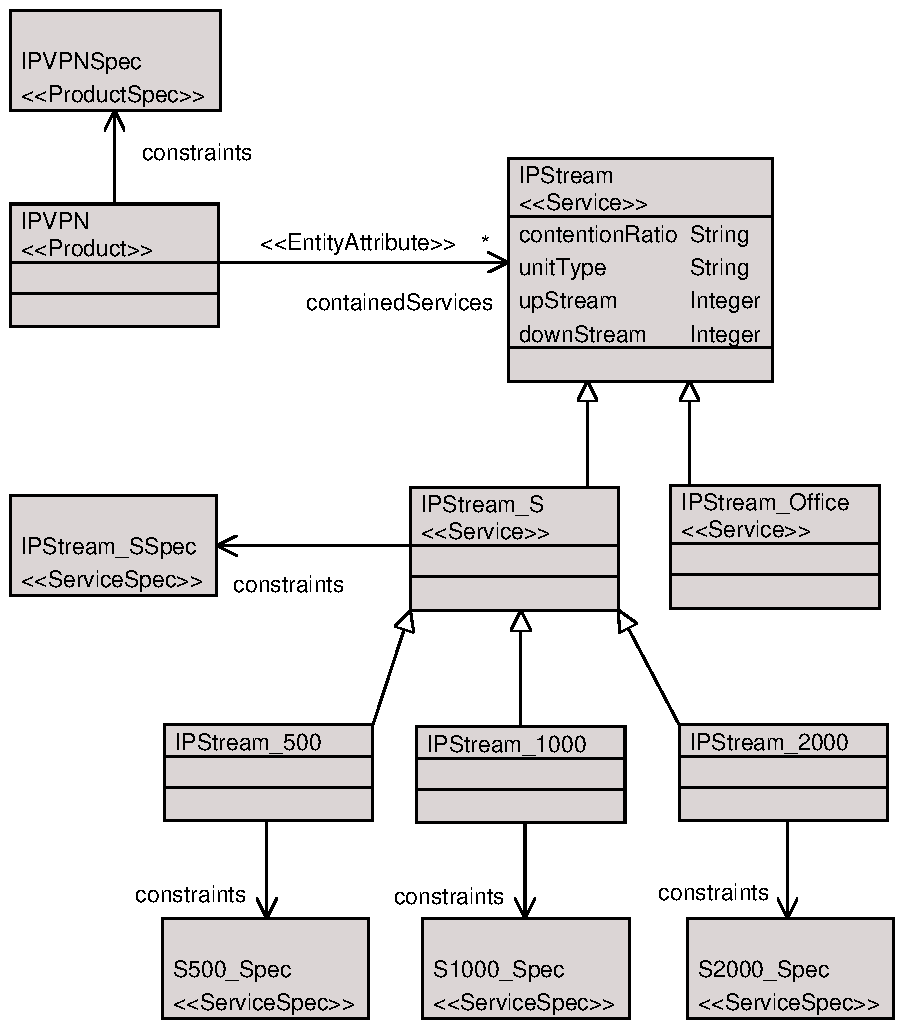
\includegraphics[width=9cm]{CaseStudy2/figures/model.pdf}
\caption{An inventory model} \label{inventorymodel}
\end{center}
\end{figure}


Because all model entities of figure \ref{inventorymodel} are
instances of inventory meta-classes that specialise Entity, which,
in turn, extends class XCore::Class, they inherit the ability to
have constraints, attributes and operations (and their associated
specialisations, namely, Specifications and EntityAttribute). As
an example, the IPStream\_S2000 is associated with S2000Spec,
which has the following XOCL body:

\begin{lstlisting}
self.upStream = 250 and
self.downStream = 2000 and
self.unitType ="kbps"
\end{lstlisting}In addition, XOCL can be used to write operations on the inventory
model. XOCL extends OCL with a small number of action primitives,
thus turning it into a programming language at the modelling
level. As an example, the following operation creates an instance
of an IPStream and adds it as a containedServices attribute to an
IPVPN:

\begin{lstlisting}
context IPVPN
  @Operation addIPStream(up,dwn,unit,con)
    self.containedServices :=
      self.containedService->including(IPStream(up,dwn,unit,con))
  end
\end{lstlisting}Finally, because the entities in the model are themselves
instantiable, it is possible to create an instance of the
IPStreamModel and check that the instance satisfies the
constraints that are defined in the inventory model (see figure
\ref{inventorysnapshot}). This is a further level of instantiation
that is possible because of the metaPackage relationship between
the inventory model and the inventory language meta-model.
Furthermore, the operations on the model can be executed, allowing
all aspects of the model to be validated.

\begin{figure}[htb]
\begin{center}
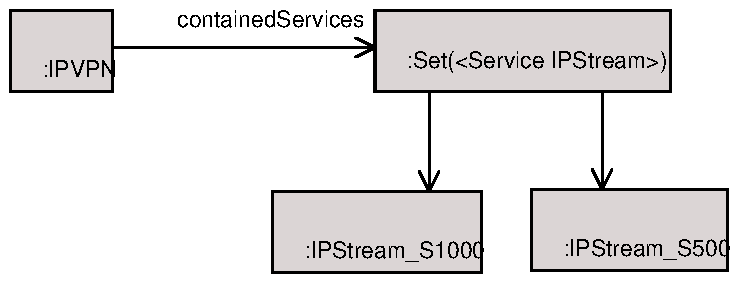
\includegraphics[width=10cm]{CaseStudy2/figures/snapshot.pdf}
\caption{A snapshot (instance) of the IPVPNModel}
\label{inventorysnapshot}
\end{center}
\end{figure}

\section{Transformations}

Using XMap, two mappings have been defined from the inventory
language. The first generates EJBs, while the second focuses on
the generation of Java and a Java class tool. We concentrate on
the second one here.

The model of figure \ref{inventorymapping} shows the mappings used
to generate Java. Rather than mapping directly from the inventory
language meta-model, a more generic approach is taken in which the
mapping was defined from XCore classes. Because the inventory
language extends the XCore meta-model, they therefore also apply
to inventory models (and any other language specialisations
defined in the future).

\begin{figure}[htb]
\begin{center}
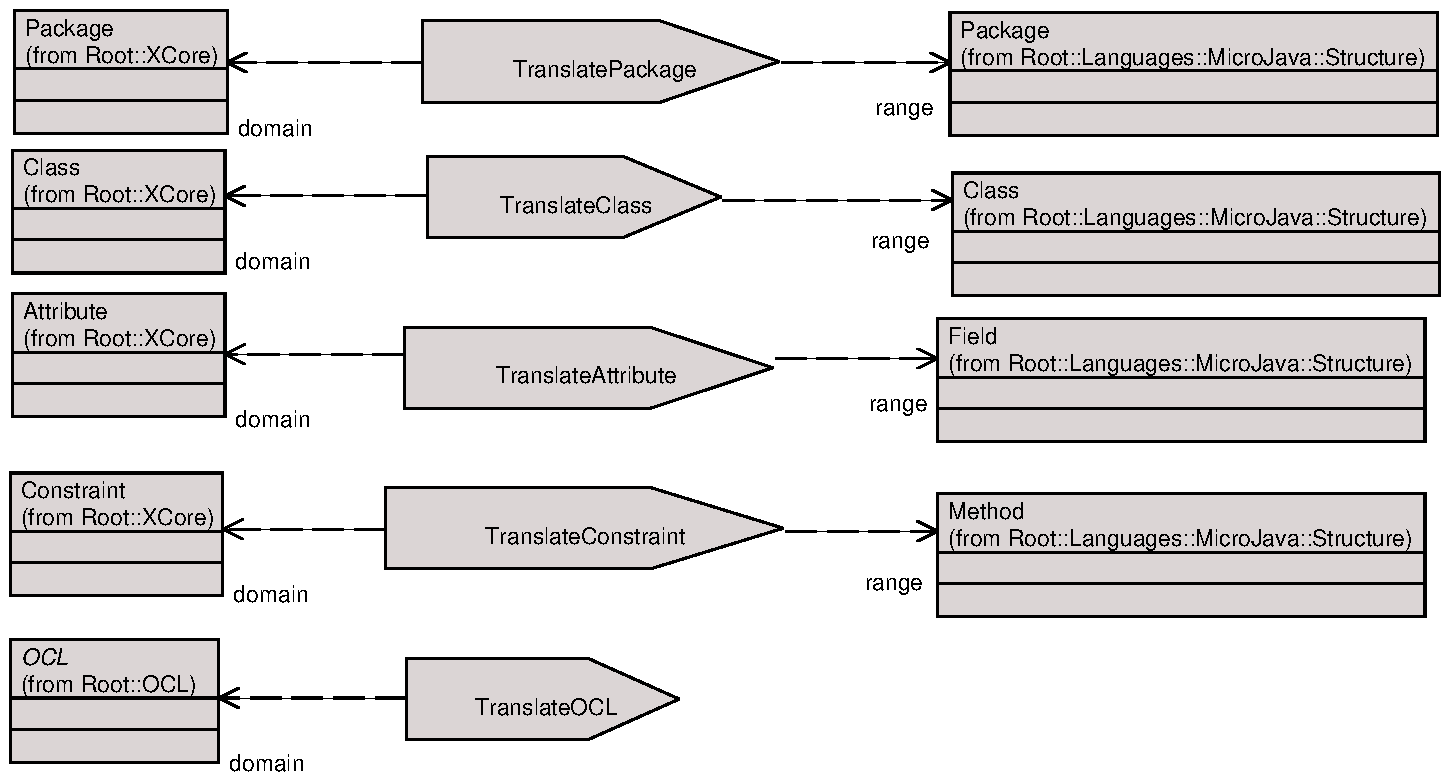
\includegraphics[width=15cm]{CaseStudy2/figures/javamapping.pdf}
\caption{Overview of the XCore to Java mapping}
\label{inventorymapping}
\end{center}
\end{figure}

Every element in the XCore package has a mapping to a
corresponding element in the Java meta-model. The following clause
describes a mapping from an XCore class to a Java class:

\begin{lstlisting}
context TranslateClass
    @Clause MapClass
      XCore::Class[name = name,
                   parents = P,
                   operations = O,
                   constraints = C,
                   attributes = A] do
      classToMicroJava(name,P,O,C,A)
    end
\end{lstlisting}Here, a Class is mapped to a Java Class, which is the result of
passing the class's name, parents, operations, constraints and
attributes into the operation classToMicroJava(). This operation
is shown below:

\begin{lstlisting}
context XCore::Class
  @Operation classToMicroJava(name,P,O,C,A)
    let K = constraintsToMicroJava(C);
        M = O->asSeq->collect(o | XCoretoMicroJava(o));
        F = A->asSeq->collect(a | XCoretoMicroJava(a))
    in if P = Set{Object}
       then [| @Java class <name> { <* F + K + M *> } end |]
       else
         let parent = P->sel.name.toString()
         in [| @Java class <name> extends <Seq{parent}> { <* F + K + M *> } end |]
         end
       end
    end
\end{lstlisting}Briefly, the operation makes use of quasi quotes (see chapter
\ref{concretechapter}) to 'drop' the name, parent and (once they
have been translated) the attributes, operations and constraints
into a syntactical definition of a Java class. This is possible
because an XBNF grammar has been defined for the MicroJava
language. The result will be an instance of the MicroJava language
metamodel, which can then outputted as a program in textual form.

An important point to make about the mapping is that it translates
all elements of an XCore model (and by specialisation and
inventory model) into Java. This includes the bodies of operations
and constraints, which are translated into Java operation. The
resulting Java program can be run and checked against the
behaviour of the original model running on the VM.

\section{Tool Mapping}

While the above mapping generates a standalone Java program
corresponding to an inventory model, it would more useful to users
of the language if the model it represents could be interacted
with via a user interface. To achieve this, a mapping was
constructed from XCore to a meta-model of a tool interface for
managing object models. This represents a domain specific language
for tools. The meta-model of the class tool interface is shown in
figure \ref{toolmodel}. A class tool provides an interface that
supports a standard collection of operations on objects, such as
saving and loading objects and checking constraints on objects. In
addition, a class tool defines a number of managers on classes,
which enable instances of classes to be created and then checked
against their class's constraints or their operations run.

\begin{figure}[htb]
\begin{center}
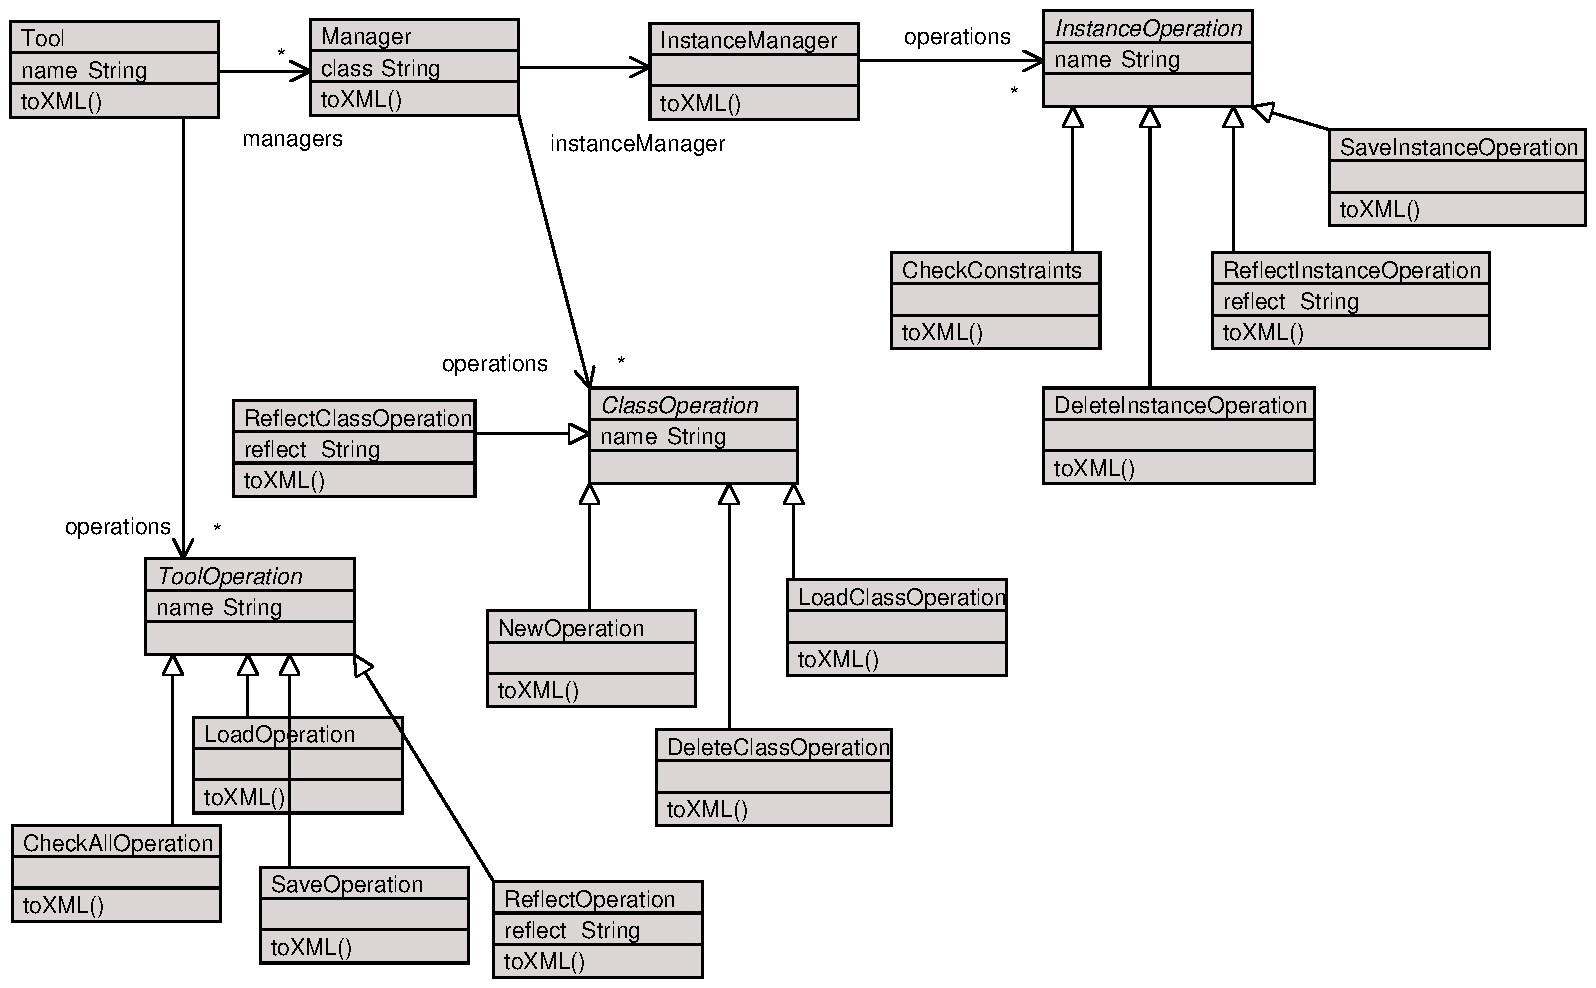
\includegraphics[width=16cm]{CaseStudy2/figures/toolmodel.pdf}
\caption{The class tool metamodel} \label{toolmodel}
\end{center}
\end{figure}

A mapping can be defined to the class tool meta-model (not shown
here), which generates a tailored user interface for creating and
manipulating instances of a meta-modelling language such as the
inventory language. Applying this mapping to the IPVPN model shown
in figure \ref{toolmodel} results in the generation of the class
tool in figure \ref{classtoolexample}. Here, buttons have been
generated for each of the entities in the model. These allow the
user to create new instances, edit their slot values and delete
instances. As the figure shows, a button for invoking the
addIPStream() method defined earlier has also been added in the
GUI executing functionality that implements in Java the method's
behaviour described in the model with XOCL.

\begin{figure}[htb]
\begin{center}
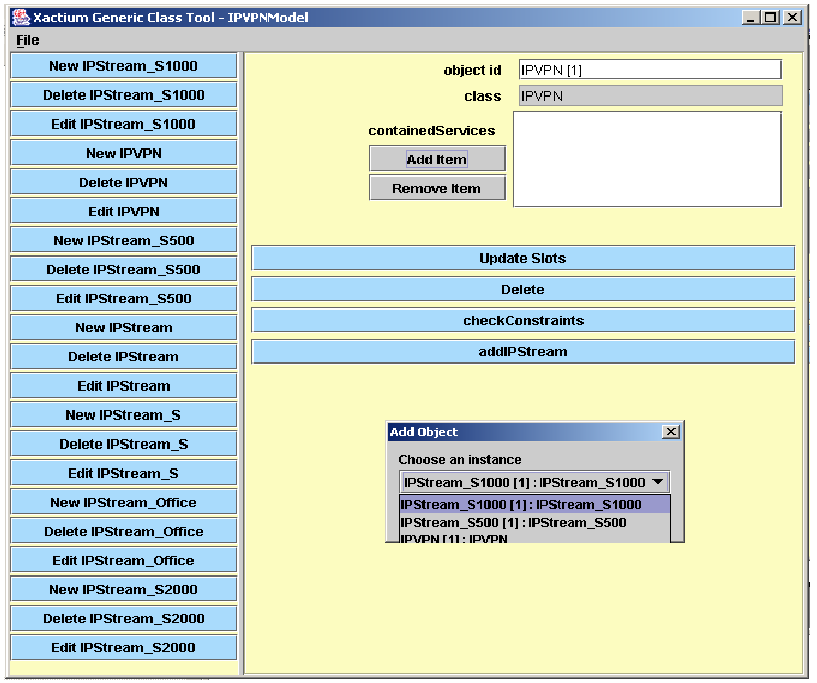
\includegraphics[width=14cm]{CaseStudy2/figures/classtoolexample.pdf}
\caption{The generated class tool} \label{classtoolexample}
\end{center}
\end{figure}

\section{Conclusion}

This chapter has shown how a relatively light weight approach to
extending a metamodel can be used to define a domain specific
modelling language. Metapackages were used to ensure consistancy
of models against its metmodel. Because of the completeness of the
new language, it was then possible to generate a complete
deployment of domain specific language in Java.
